\draft Classic GHZ question.

\begin{parts}
	\part \todo Noting that vertical and horizontal polarisations are orthogonal, we make identification:
	\begin{equation*}
		\ket{0} \equiv \ket{\mathrm{H}} \qquad \ket{1} \equiv \ket{\mathrm{V}}
	\end{equation*}
	
	The states $\ket{\pm}$ are then $\ket{\mathrm{H}} \pm \ket{\mathrm{V}}$, i.e. polarisation $45\degree$ to horizontal/vertical.
	
	Similarly, $\ket{R}$ and $\ket{L}$ are $\ket{\mathrm{H}} \pm i\ket{\mathrm{V}}$, i.e. right/left handed polarisation.
	
	A Hadamard gate may be achieved by placing a $\pi$ waveplate $22.5\degree$ to horizontal as shown below:
	\begin{figure}[H]
		\centering
		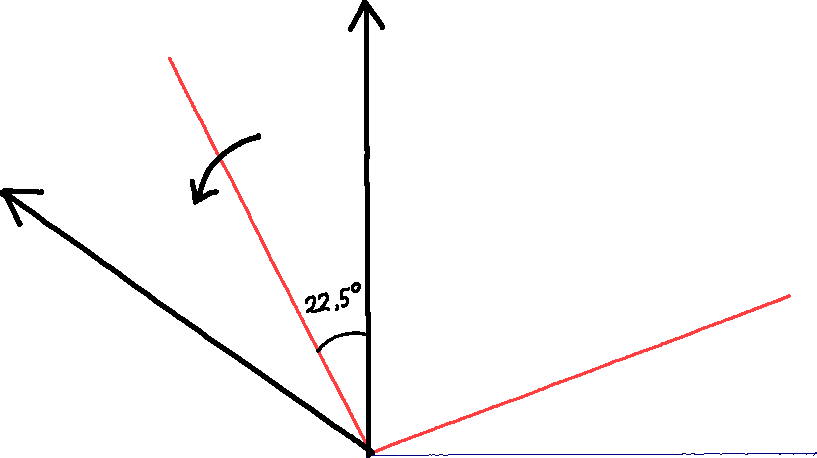
\includegraphics[width=.7\linewidth]{q7-hadamard}
	\end{figure}
	
	A controlled phase gate may be achieved by adjusting the angle and phase of a waveplate by Pockels effect.
	The control should come from?
	
	The main reasons why a 2-photon gate in such basis is difficult to implement is due to its sensitivity to polarisation angle, a slight error could render the gate unusable.
	
	\part Ignoring normalisation:
	\begin{align*}
		\ket{000} &\xrightarrow{\mathrm{H}^{\otimes 3}} \ket{+++} = \ket{000} + \ket{001} + \ldots + \ket{111} \\
		&\xrightarrow{\mathrm{CZ}_{13}} \ket{000} + \ldots + \ket{100} - \ket{101} + \ket{110} - \ket{111} \\
		&\xrightarrow{\mathrm{CZ}_{12}} \ket{000} + \ldots + \ket{100} - \ket{101} - \ket{110} + \ket{111} = \ket{0}\ket{++} + \ket{1}\ket{--} \\
		&\xrightarrow{\mathds{1} \otimes \mathrm{H}^{\otimes 2}} \ket{000} + \ket{111}
	\end{align*}
	So we have generated a GHZ state in the ZZZ basis.
	
	To rewrite the GHZ state in other bases, we first note the following transformations:
	\begin{align*}
		\ket{0} &= \frac{\ket{+} + \ket{-}}{\sqrt{2}} \mtext{in X basis} &= \frac{\ket{R} + \ket{L}}{\sqrt{2}} \mtext{in Y basis} \\
		\ket{1} &= \frac{\ket{+} - \ket{-}}{\sqrt{2}} \mtext{in X basis} &= \frac{\ket{R} - \ket{L}}{\sqrt{2}} \mtext{in Y basis up to a global phase of $i$}
	\end{align*}
	
	So we may rewrite the GHZ state as:
	\begin{align*}
		\ket{\textnormal{GHZ}} &= \rbracket{\ket{+} + \ket{-}} \rbracket{\ket{R} + \ket{L}} \rbracket{\ket{R} + \ket{L}} + \rbracket{\ket{+} - \ket{-}} \rbracket{\ket{R} - \ket{L}} \rbracket{\ket{R} - \ket{L}} \\
		&= \ket{+RR} + \ket{+RL} + \ket{+LR} + \ket{+LL} + \ket{-RR} + \ldots + \\
		&\quad \ket{+RR} - \ket{+RL} - \ldots + \ket{+LL} - \ket{-RR} + \textnormal{cross terms} - \ket{-LL} \\
		&= \ket{+}\sbracket{\ket{RR} + \ket{LL}} - \ket{-}\sbracket{\ket{LR} + \ket{RL}} \mtext{in XYY basis}
	\end{align*}
	
	Similarly we have:
	\begin{align*}
		\ket{\textnormal{GHZ}} &= \ket{R+R} + \ket{L+L} - \ket{L-R} - \ket{R-L} \mtext{in YXY} \\
		&= \sbracket{\ket{RR} + \ket{LL}}\ket{+} - \sbracket{\ket{LR} + \ket{RL}}\ket{-} \mtext{in YYX}
	\end{align*}
	
	Note that there is an entanglement between the X and Y pairs -- if Y is measured to be the same $\Rightarrow$ X must be $\ket{+}$ and vice versa.
	
	In XXX basis:
	\begin{align*}
		\ket{\textnormal{GHZ}} &= \rbracket{\ket{+} + \ket{-}}^{\otimes 3} + \rbracket{\ket{+} - \ket{-}}^{\otimes 3} \\
		&= \ket{+++} + \ket{+--} + \ket{--+} + \ket{-+-} \textnormal{\hspace{.5em}noting that odd powers of $\ket{-}$ cancels} \\
		&= \ket{+}\ket{\Phi^+} + \ket{-}\ket{\Psi^+}
	\end{align*}
	
	Hence a measurement in X basis reveals a maximally entangled state, which is known for violating the CHSH inequality, i.e. $B = 2\sqrt{2} > 2$ as predicted by local realism.
	
	However the slight difference is that the Bell state is encapsulated in the GHZ state when measured in X basis, as opposed to being an inherent feature in computational basis.
\end{parts}